%\subsection{Metric Evaluations}
% The results are shown in figure 3
% Experiments are as discussed in Section
% The maps are as show in figure 4
\begin{figure}%
  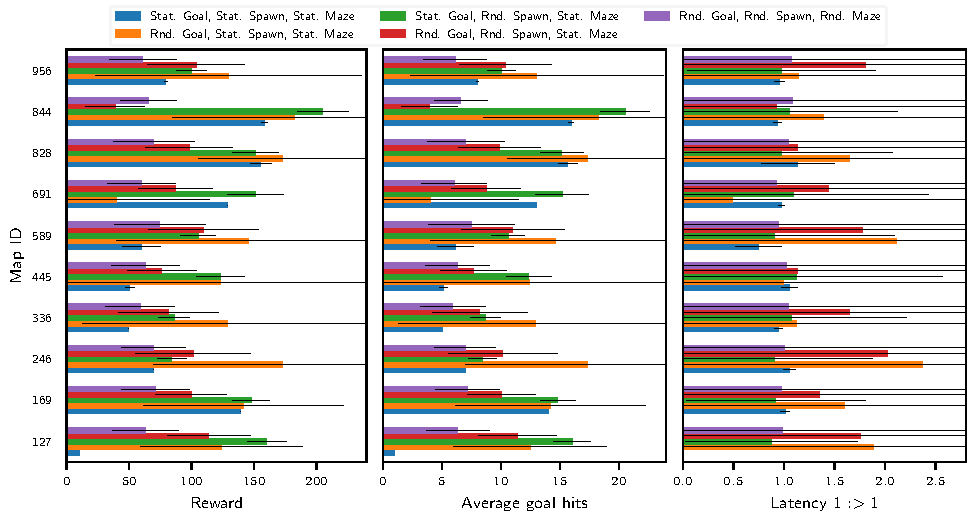
\includegraphics[width=\linewidth]{images/plot_summary_bar_plots.pdf}%
  \vspace{-1em}%
  \caption{
    We evaluate the \NavAiiiCDiDiiL{}~\cite{MiPaViICLR2017} algorithm on ten randomly chosen maps with increasing difficulty as described in Sec~\ref{sec:navtasks}.
  Vertical axis is one of the ten maps on which the agent was trained and evaluated.
  Horizontal axes are different evaluation metrics.
  We note that when the goal is static then rewards are consistently higher as compared to random goal while static spawn location and random spawn location are roughly close to each other within bounds of uncertainity. As expected, switching each variable from static to random increases the standard deviation on the results.
  From the \LatencyOneGtOne{} results we note that the current state of art algorithms do well when trained and tested on the same map but fail to generalize to new maps when evaluated on ability to exploit the information about goal location.
  Also note that \LatencyOneGtOne{} metric for cases of static goals is expected to be close to one because the location of goal is learned at train time.
  }%
\label{fig:latency-goal-reward}%
\end{figure}

In this section we discuss the results for experiments as discussed in Section~\ref{sec:navtasks} over the ten randomly chosen maps shown in Fig~\ref{fig:environments}. The results are in Fig~\ref{fig:latency-goal-reward}.
\paragraph{Static goal, static spawn, static maze}
For this case, the reward is consistently high, and \DistanceInefficiency{} is close to 1 with small standard deviations implying the path chosen is the shortest available.
Please note that \LatencyOneGtOne{} should be close to 1 for the static goal case because the goal location is known at training time.

\paragraph{Static goal, random spawn, static map}
Again, note that \DistanceInefficiency{} is close to 1 implying that when the goal is found, the shortest path is traversed.
This is because the agent can learn the optimal  policy for the shortest path to the goal at training time.

\paragraph{Random goal, static spawn, static map}
In this case, the mean of the \LatencyOneGtOne{} is more than 1 showing that in general the agent is able to exploit map information.
However the large standard deviations in this metric and the reward values show that this exploitation is not consistent through episodes.
For most of the experiments, the \DistanceInefficiency{} is close to one within error metrics, again implying that the shortest path is taken when the goal is found. 

\paragraph{Random goal, Random spawn, static map}
Similar to the previous experiment, the \LatencyOneGtOne{} is more than 1 but with a large standard deviation implying inconsistent performance from episode to episode.
The \DistanceInefficiency{} is larger than 1 showcasing the paths traversed to the goal are not necessarily the shortest.

\paragraph{Random goal, Random spawn, Random map}
For this experiment, agents trained on a 1000 maps are tested individually on the 10 chosen maps that are a subset of the 1000 maps.
The \LatencyOneGtOne{} is close to 1 implying that map-exploitation not is taking place.
The large \DistanceInefficiency{} numbers seem to confirm this statement.
We present, qualitative results in  Sec.~\ref{sec:qualitative-simple} on very simple maps to show that the agents are only randomly exploring the maze rather than utilizing any form of shortest path planning.

\subsection{Evaluation on unseen maps}
The results for training on $N$ maps, where $N \in \{10, 100, 500, 1000\}$, and testing on 100 unseen maps are shown in Fig~\ref{fig:num-training-maps}.
We observe that there is a significant jump of average reward and average goal hits when the number of training maps is increased from 10 to 100 but no significant increase when the number of training maps are increased from 100 to 500 to 1000.
This is due to the fact that the wall-following strategy learned by the algorithm,
is learned with enough variation in 100 maps and training on additional maps does not add to the learned strategy.

\subsection{Effect of apples and texture}
We evaluate the effect of apples and textures during evaluation time in Fig~\ref{fig:num-training-maps}.
We train the algorithm on randomly chosen training maps with random textures and evaluate them on maps with and without random textures and also with and without apples. 
We find that the algorithm, being trained on random textures and the random placement of apples is robust to the presence or absence of textures and apples.


\subsection{Qualitative evaluation on simple maps}
\label{sec:qualitative-simple}
% 1. We test the trained algorithms on simple maps.
To evaluate what strategies the algorithm is employing to reach the
goal we evaluate the algorithm on very simple maps where there are only two
paths to reach the goal. The qualitative results for the evaluation are shown
in Fig~\ref{fig:planning-qualitative}.

\begin{figure}%
  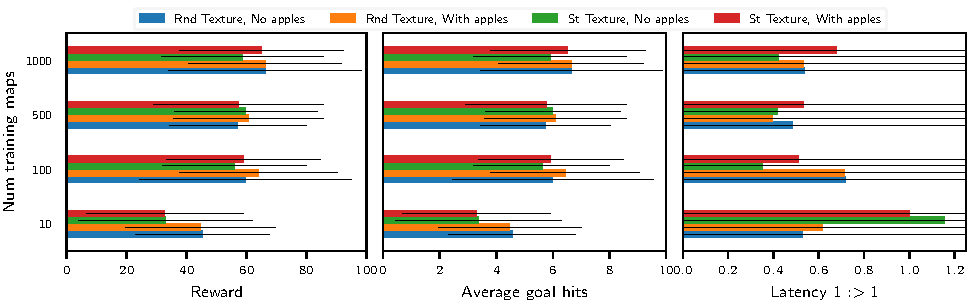
\includegraphics[width=\linewidth]{images/plot_ntrain_summary.pdf}%
  \caption{Plots showing the effect of number of training maps with random texture (Rnd Texture) and presence of apples (With apples), when evaluated on unseen maps. We note that although the difference between mean metrics is negligible as compared to standard deviation of the metrics. Hence we say that the effect of apples or textures can be ignored.
  The only clear trend is apparent \LatencyOneGtOne{} metric which suggest that random texture along without apples is advantageous in exploiting goal location while finding the goal second time on-wards.}
  \label{fig:num-training-maps}
\end{figure}

\paragraph{Square map}
% 3. In the square map, we find that the path taken is in the
%    direction of pose initialization. the visualization of path taken is
%    shown in Fig. . the correlation with of path taken with initial pose
%    is shown in Fig. . The correlation with shortest path is shown in
%    Fig. . Hence, the algorithm instead of shortest path planning takes the
%    the direction in which it is initialized.
A Square map (Fig~\ref{fig:planning-qualitative}) is the simplest possible map with two paths to the goal.
We evaluate the algorithm trained on 1000 random maps on this map.
We observe that the agent greedily moves in the direction of
initialization.
This may be because of the initial learning which is
motivated by small rewards of getting apples.
We compute the percentage of times the agent takes the shortest path over a trial of 100 episodes.
We find the agent takes the shortest path only $50.4$\% ($\pm 12.8$\%) of the times which is no better than random.
% Quantitative result taken from:
% exp-results/planning-09x09-0002/gen_stats_latest_loaded-from-training-1000_acting-on-planning-09x09-0002_vars-True_apples-0.json

\paragraph{Wrench map}
% 2.2 To eliminate the correlation with initial orientation, we start
%     with wrench map. The spawn point is guaranteed to be initialized in
%     the handle of the wrench. Hence, the decision point is the only
%     junction in the map where the algorithm either decides to take a
%     left or a right.
%     We find no correlation between shortest path and the direction taken. 
To eliminate the dependency on initial orientation, we evaluate the algorithm on Wrench map as shown in Fig~\ref{fig:planning-qualitative}. We fix in the spawn point at the bottom of the tail so that shortest path is independent of the spawn orientation.
The decision about the shortest path is made at the junction where the agent can either chose to go left or right.
We find that the agent takes the shortest path only $32.9$\% ($\pm 25.1$\%) of the times which is in fact worse than random.
% Quantitative result taken from:
% exp-results/planning-09x09-0004/gen_stats_latest_loaded-from-training-1000_acting-on-planning-09x09-0004_vars-True_apples-0.json

% Goal map provides a similar independence from starting orientation
% but the penalty for choosing the wrong path is much higher than the
% wrench map. 
\paragraph{Goal map}
Similar to the wrench map, the goal map (Fig~\ref{fig:planning-qualitative}) provides a decision point independent of the initial orientation but penalizes the wrong decision more than the wrench map. The shortest path is chosen $42.6$\% ($\pm 35.1$\%) of the times which is again no better than random.
% Quantitative result taken from:
% exp-results/planning-09x09-0006/gen_stats_latest_loaded-from-training-1000_acting-on-planning-09x09-0006_vars-True_apples-0.json

% JJC: TODO: Summarize results on simple maps
These experiments show that \NavAiiiCDiDiiL{} algorithm, even when trained on 1000 maps, do not generalize to these very simple maps.
Again note that even in cases when there are only two possible paths to the goal, the agent is unable to chose the shorter path with more than 50\% probability.
This shows that the models trained on 1000 maps have learned only a wall-following strategy rather than a learning to plan-path based one.

%\subsubsection{Qualitative results}
\begin{figure}[h]
\def\vertspace{1ex}
\rotatebox{90}{\hspace{1ex}\tiny Square map}%
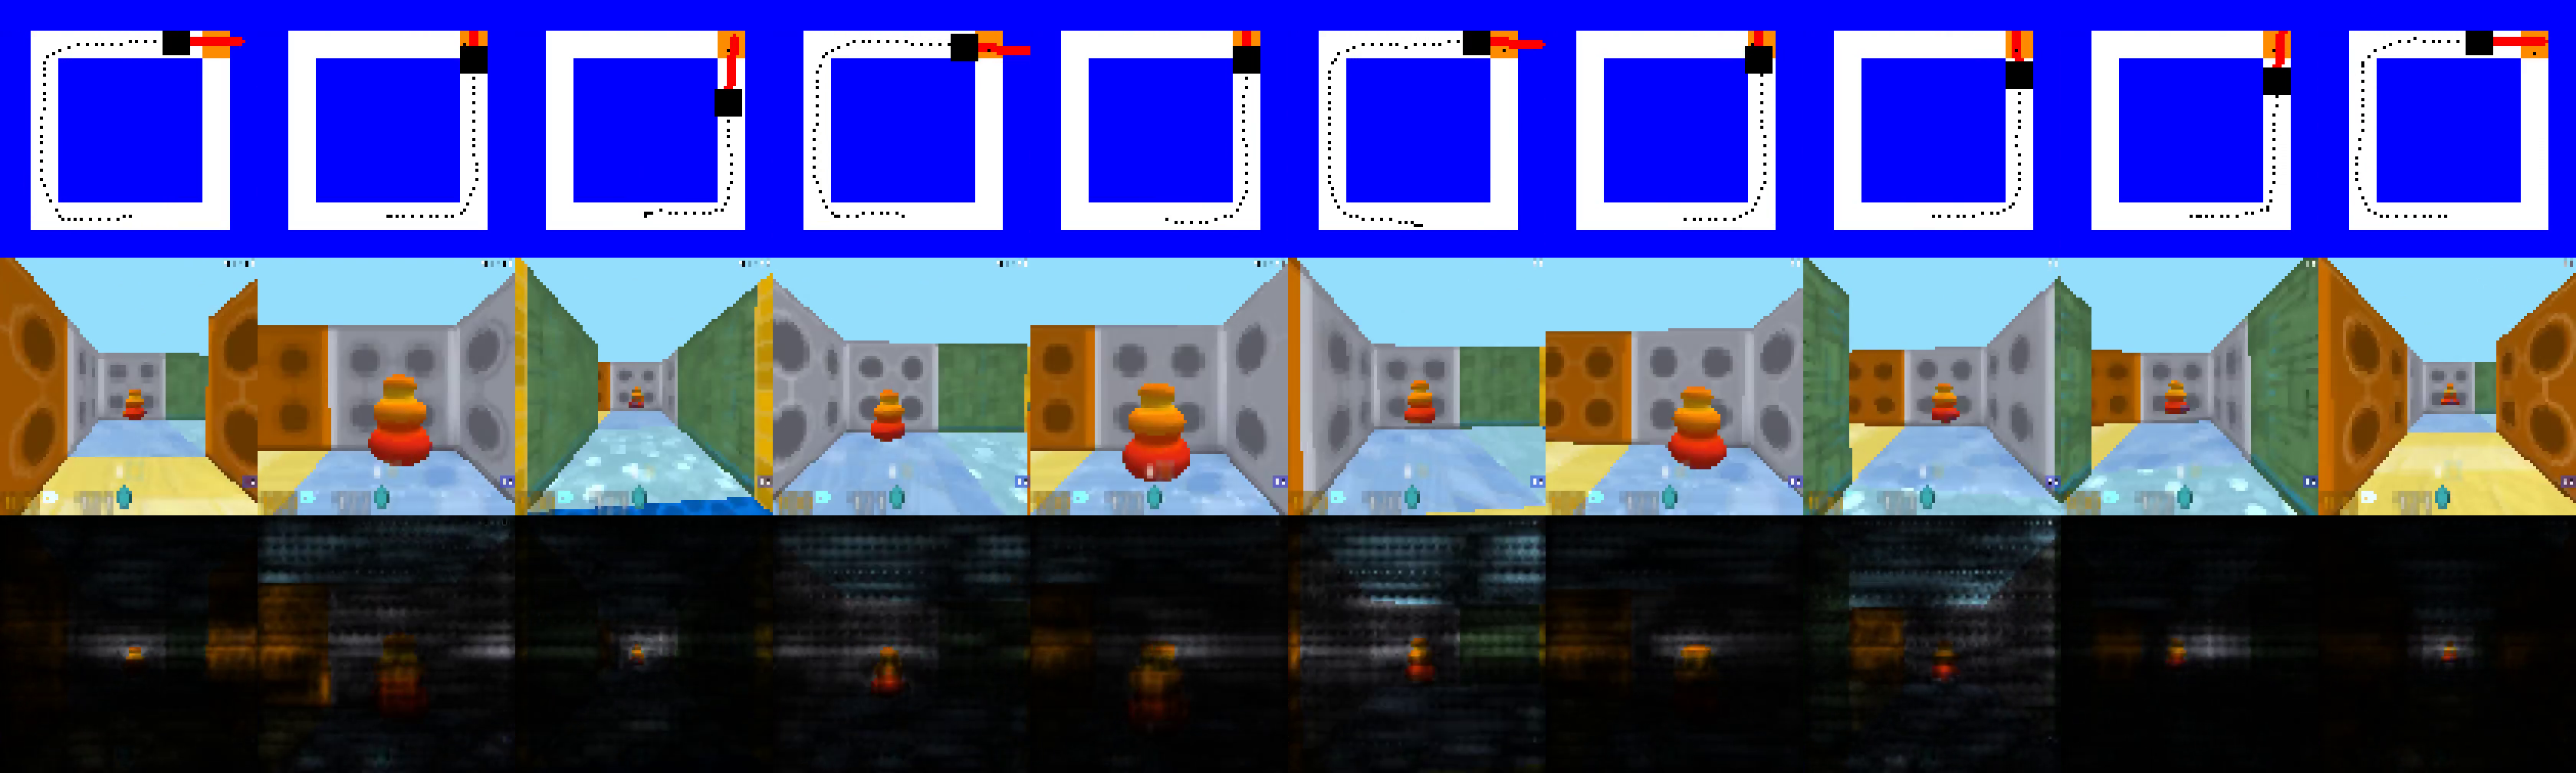
\includegraphics[width=0.98\textwidth,trim=0 672pt 0 0,clip]{./exp-results/training-1000_on_square_map.png}%
\vspace{\vertspace}
\rotatebox{90}{\hspace{1ex}\tiny Wrench map}%
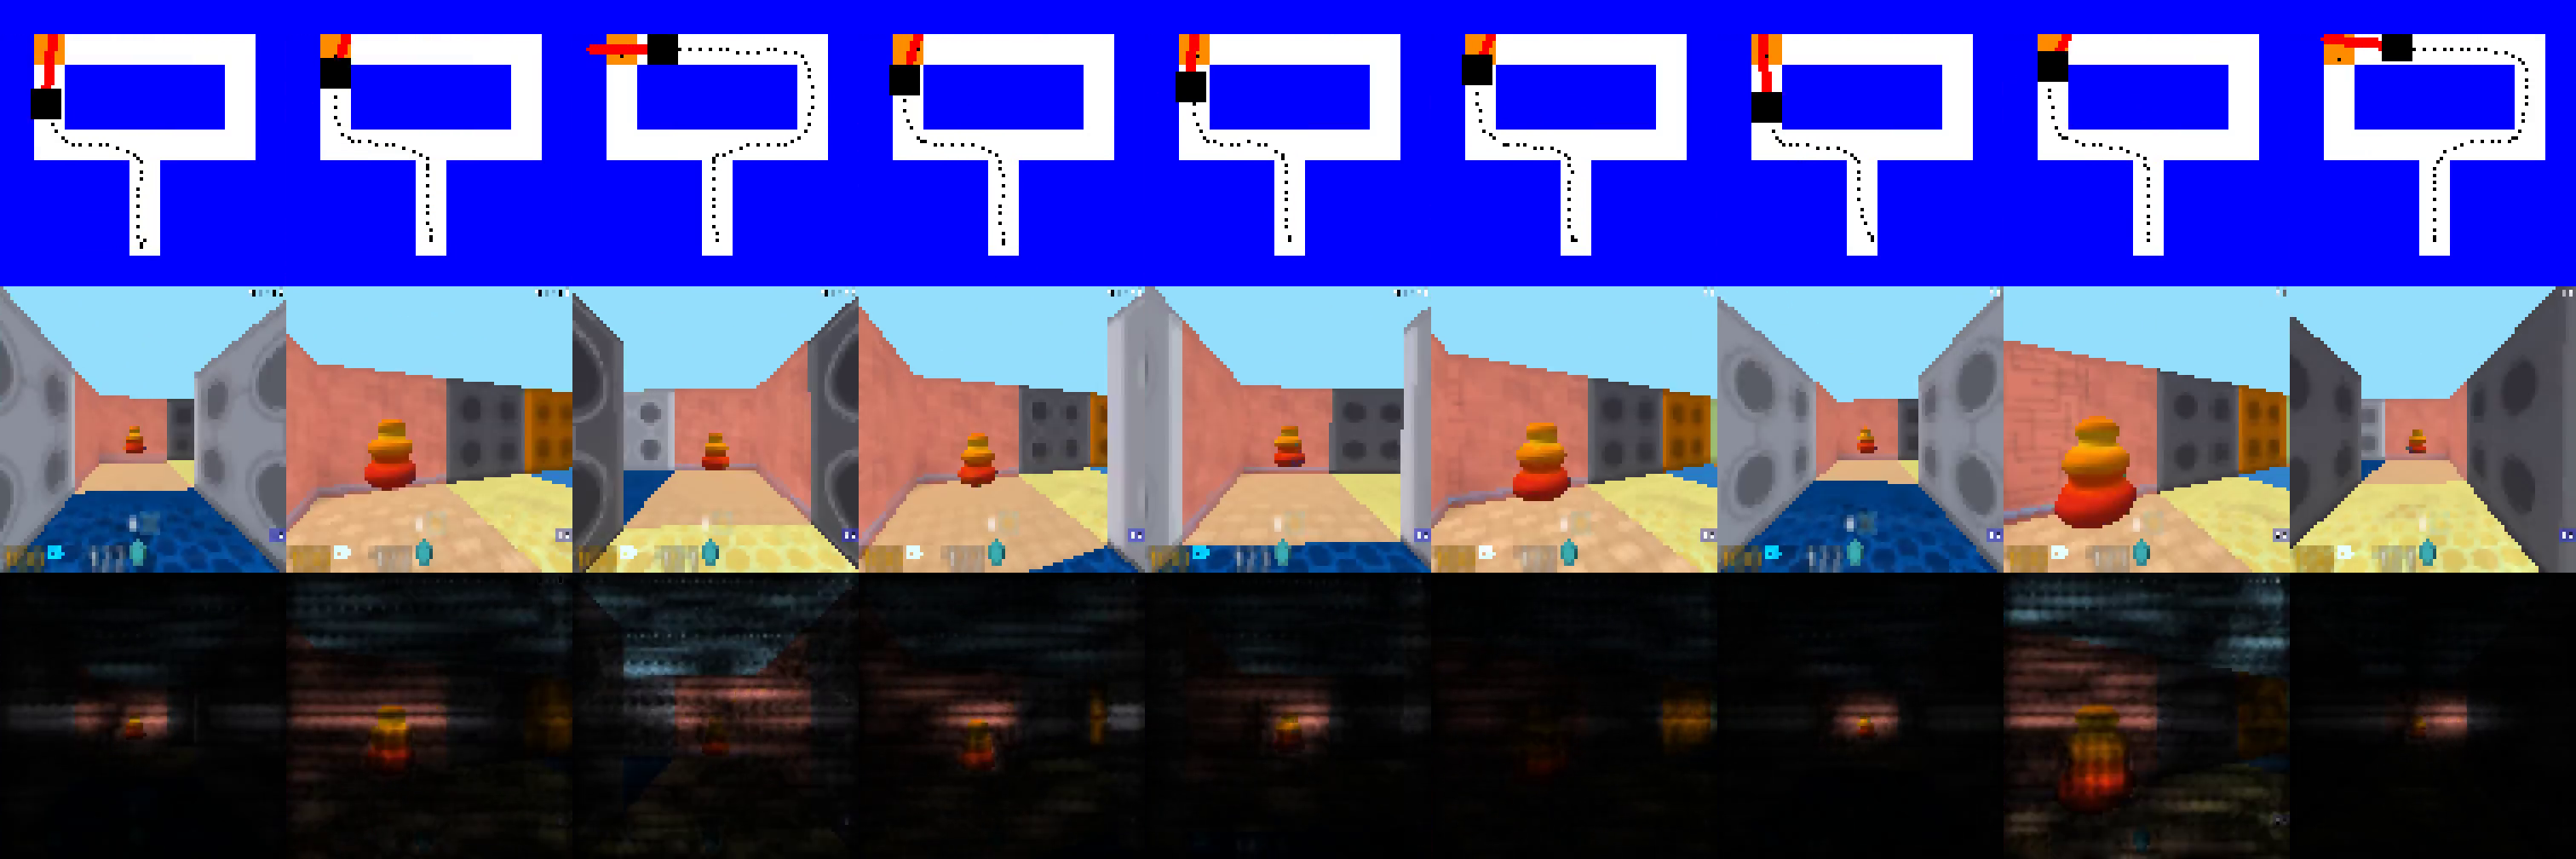
\includegraphics[width=0.98\textwidth,trim=0 672pt 0 0,clip]{./exp-results/training-1000_on_wrench_map.png}%
\vspace{\vertspace}
\rotatebox{90}{\hspace{2ex}\tiny Goal map}%
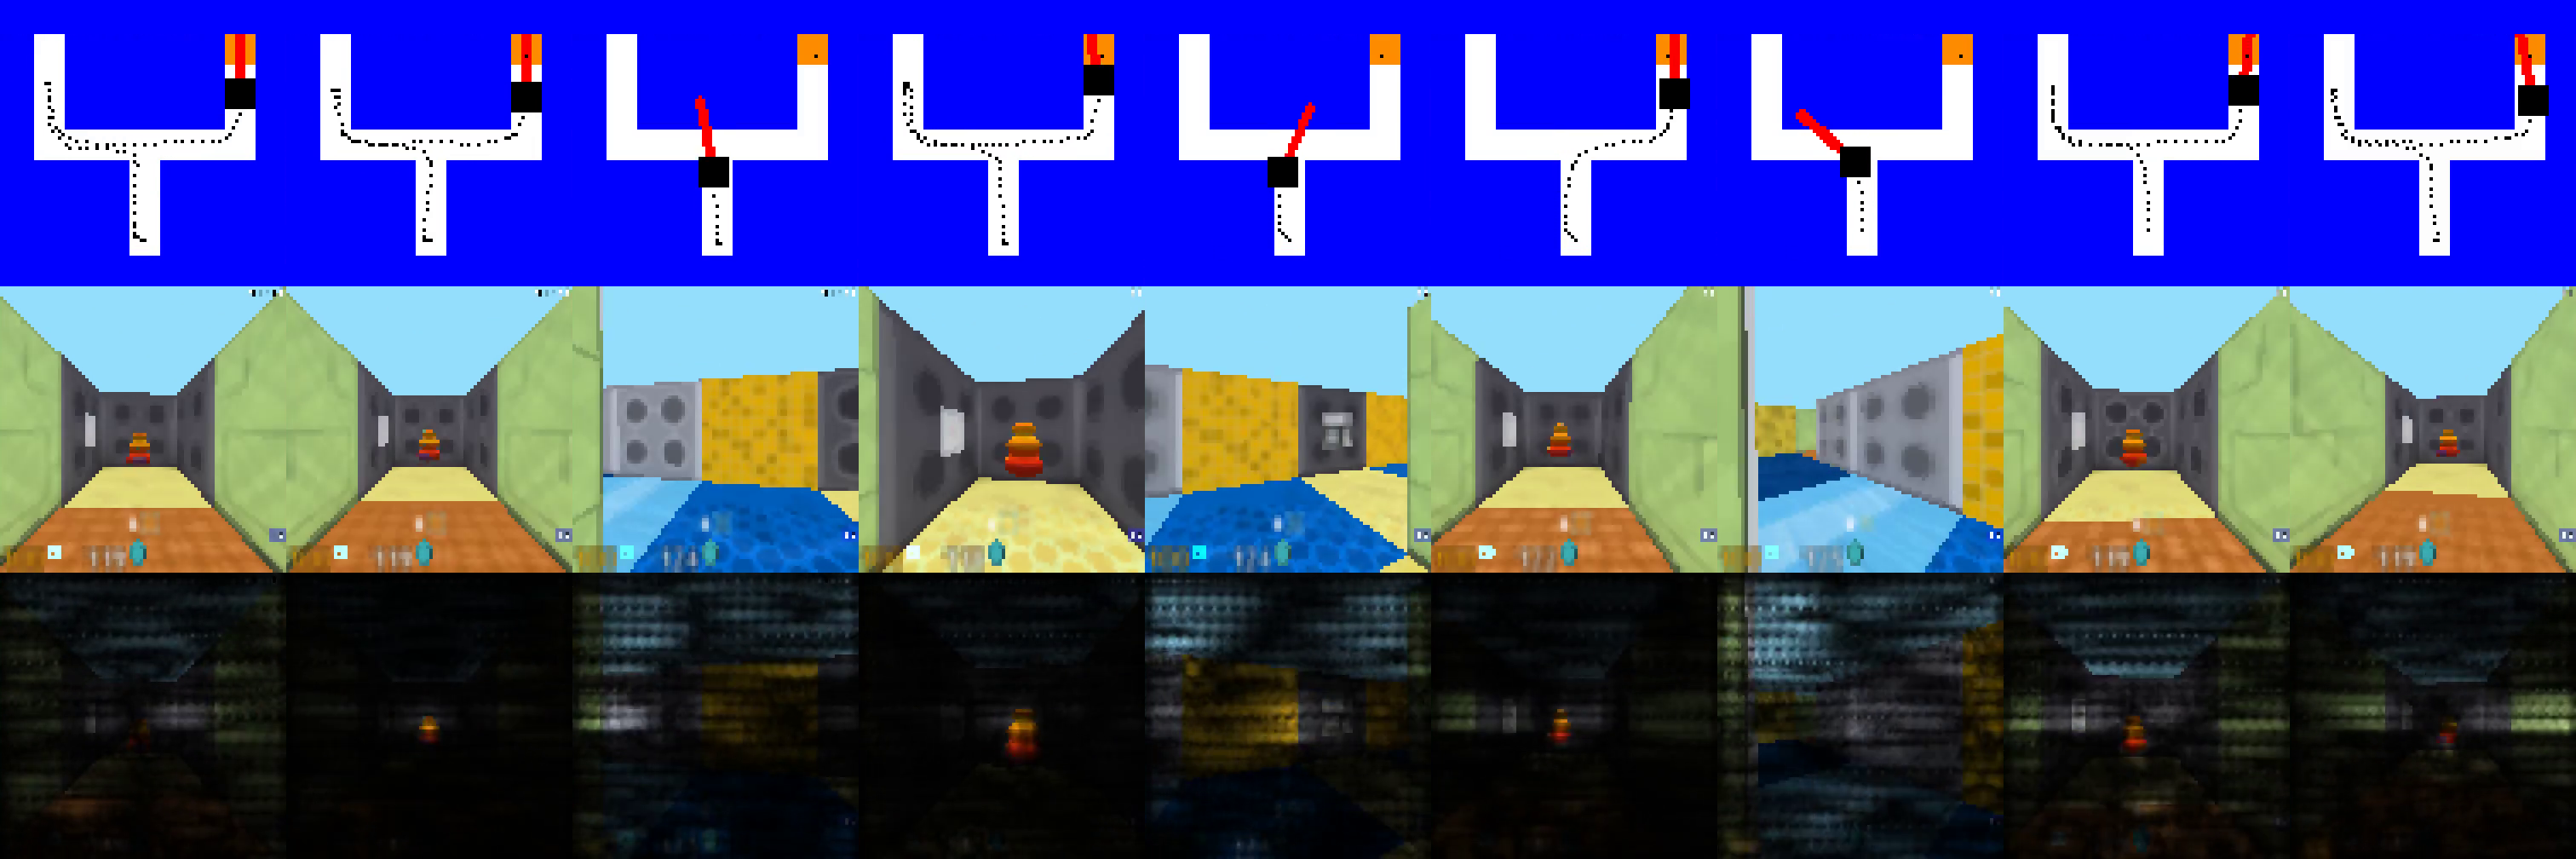
\includegraphics[width=0.98\textwidth,trim=0 672pt 0 0,clip]{./exp-results/training-1000_on_goal_map.png}%
\caption{Snapshots of path taken by the agent to reach the goal in a single episode when model trained on 1000 maps is evaluated Square, Wrench and Goal map.
  The top row shows an evaluation example on Square map, the agent takes the shortest path 6/10 times but when averaged over 100 episodes, the percentage of shortest path taken is not better than random $50.4$\% ($\pm 12.8$\%).
  Although for the example of Wrench map the agent takes the shortest path 8/10 times but when averaged over 100 episodes, the percentage of shortest path taken is reduced to $32.9$\% ($\pm 25.1$\%).
 For the Goal map, the example chosen here shows that the shortest path is only taken 1/6 times, on an average over 100 episodes, the shortest path is taken $42.6$\% ($\pm 35.1$\%) times.
}
\label{fig:planning-qualitative}
\end{figure}


\subsection{Attention Maps}
We use the normalized sum of absolute gradient of the loss with respect to the input image as a proxy for attention in the image.
The gradients are normalized for each image so that the maximum gradient is one. The attention values are then used as a soft mask on the image to create the visualization as shown in Fig~\ref{fig:attention}

We observe that the attention is uniformly distributed on the image when the agent spawns. The attention narrows down to a few pixels in the center when the agent is navigating through the corridor. It spreads to the entire image around turns and junctions. The attention also pays close attention to important objects like goal, apples and unique decals.

\begin{figure}
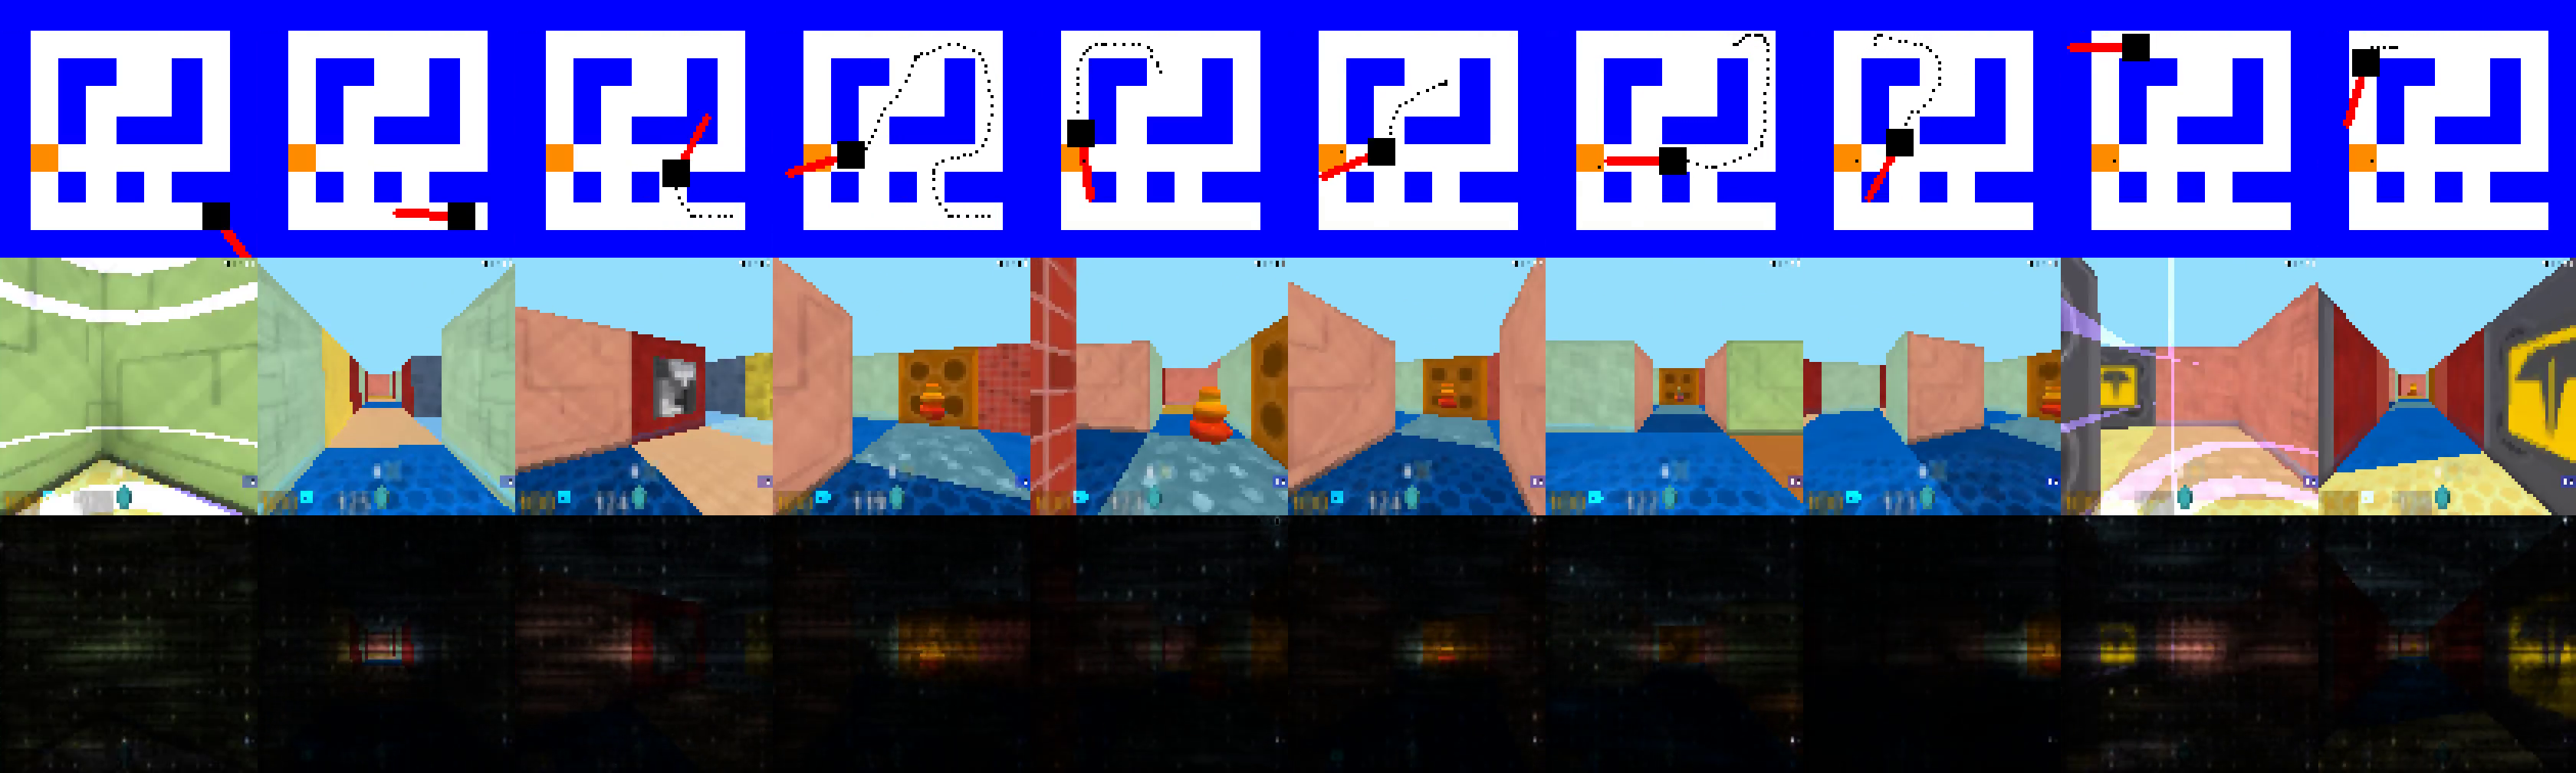
\includegraphics[width=\textwidth,trim=0 0 0 336pt,clip]{./exp-results/training-09x09-0127-on-0127.png}\vspace{1ex}\\
%
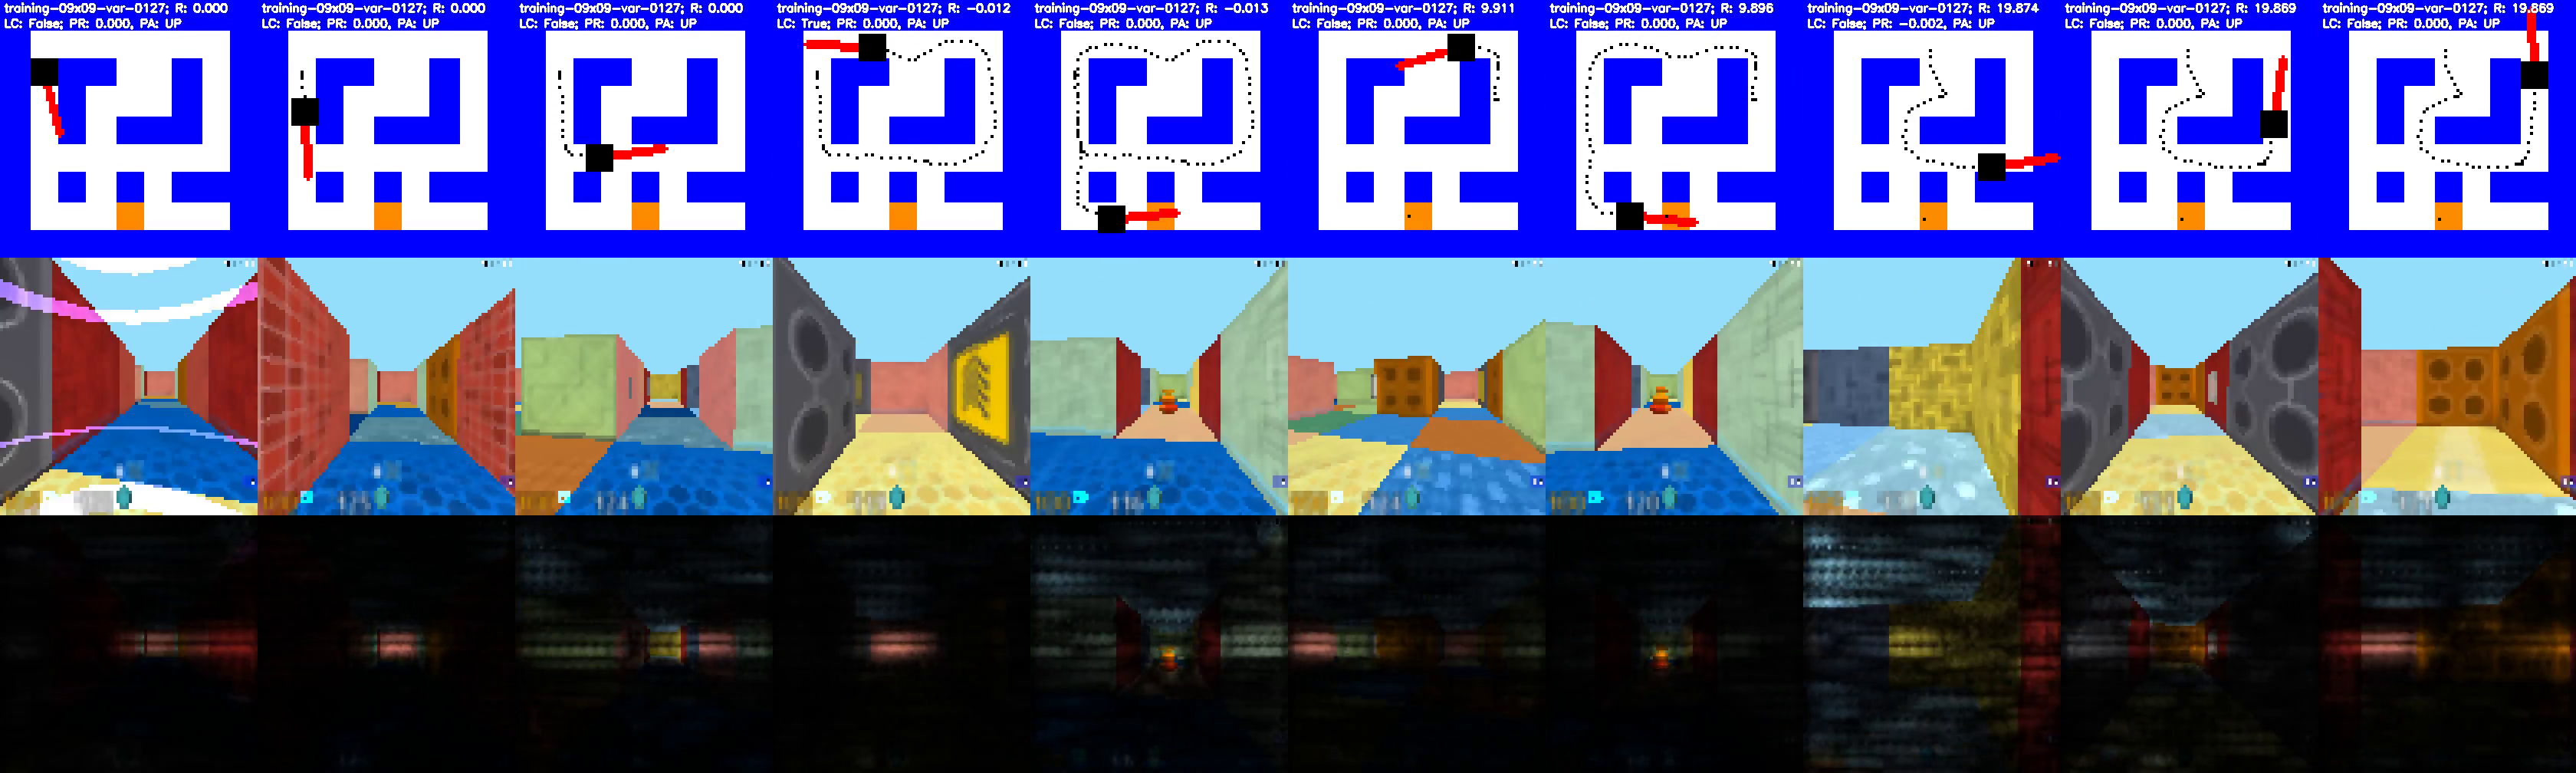
\includegraphics[width=\textwidth,trim=0 0 0 336pt,clip]{./exp-results/training-1000-on-0127.png}%
\caption{Visualizing attention for two sequences. The first two rows show the sequin when the model is trained on and evaluated on the same map. The last two rows shows the sequence for a model trained on 1000 maps and evaluated on one of the maps. We observe that the attention is uniformly distributed on the image when the agent spawns. The attention narrows down few pixels in the center when the agent is navigating through the corridor. It spreads to the entire image around turns and junctions. The attention also pays close attention to important objects like goal, apples and unique decals.}
\label{fig:attention}
\end{figure}


%Are we close to replacing the classic mapping and path-planning algorithms with DRL algorithms?
%
%As shown by the results in Fig~\ref{fig:latency-goal-reward}, the state of art DRL algorithm works well if trained and tested on the same map (static map), but performance reaches to the level of simple bug exploration like algorithms if training and testing are on different maps.



